\documentclass[sigconf, 11pt]{acmart}

\settopmatter{printacmref=false} % Removes citation information below abstract
\renewcommand\footnotetextcopyrightpermission[1]{} % removes footnote with conference information in first column
\pagestyle{plain} % removes running headers

\usepackage{booktabs} % For formal tables
\usepackage{color}
\usepackage{float}
\usepackage{graphicx}
\usepackage{caption}
\usepackage{subcaption}
\usepackage{array}
\setcopyright{none}
\usepackage{hyperref}
%\setlength\parskip{1em plus 2pt}


\begin{document}
\title{Exploring Machine Learning Prediction for Soccer Outcomes}


\author{Ryan Baker}
\affiliation{%
  \institution{University of Utah}
}
\email{u0724394@utah.edu}

\author{Nathan Wilkinson}
\affiliation{%
  \institution{University of Utah}
}
\email{u0295388@utah.edu}


\begin{abstract}

We attempted to create a predictive model for soccer games based on detailed statistics scraped from the web. Our hypothesis was that by the use of detailed statistics we could make more accurate predictions that those based on simple statistics like win percentage for each team. We found that... . Limitations. Future Work.
 
\end{abstract}

\maketitle

\section{Introduction} 

Sports betting is a common activity among sports enthusiasts around the world. In this setting, it is desirable to be able to predict the outcome of matches between two given teams. Typically, sports analysts and experts gather rich sets of data on each and every game for individual teams, and sometimes gather data on individual players. In this project we will be focusing on the problem of predicting the outcome of soccer matches, which can be used in the sports betting arena. While it can be difficult for humans to accurately predict the outcome of a match, we explore whether or not it is possible to predict outcomes accurately using machine learning techniques. While it is applicable to sports betting, it is also interesting to consider whether or not machine learning can predict outcomes, even in the presence of intangible elements of the game, such as team chemistry, home-field advantage, winning- and losing-streaks, player transfers and injuries, and other factors.

The methods utilized in this project explore a variety of algorithms, such as support vector machines (SVM), logistic regression, bagged forests, and perceptron. A large portion of this work is exploration with features, such as comparing raw statistics against derived features. We also explore the divisions of training and test data, such as comparisons between chronologically split data and randomly split data. The main lessons we learned from this project are the following:

\begin{enumerate}
\item Feature selection and the relevance of data is extremely important and can significantly impact machine learning model performance.
\item The selections of concept class and hypothesis space are important aspects of machine learning pursuits and can heavily impact the performance of a model. That is, the bias introduced by the best hypothesis in the space can be a significant limiting factor and must be monitored and controlled carefully.
\end{enumerate}

\section {Related Work and Background}
Sports betting is a common activity among avid sports fans in all sports, including soccer, basketball, football, baseball, and many other sports. To facilitate betting, many organizations publish public betting lines that describes which team is favored to win a game, and how much they are favored to win a game. However, many, or perhaps even most, of these models are strictly statistical and probabilistic. We seek to apply machine learning. Our goal is to focus on soccer, particularly in the United States, and to explore how different algorithms may produce better results, and if different train/test splits on data have an impact on learning results (e.g. explore if it is more useful to split data randomly or linearly within the course of a single season).

We have explored several different studies of machine learning with sports betting. These studies explore data from NCAA (college) basketball in the United States \cite{zimmermann2013predicting}, NFL (professional) football in the United States \cite{warner2010predicting}, and EPL (professional) soccer in England \cite{constantinou2012pi}. These reports have utilized Bayesian methods \cite{constantinou2012pi, zimmermann2013predicting}, decision trees and random forests \cite{zimmermann2013predicting}, and Gaussian processes \cite{warner2010predicting}. An important common aspect of all of these studies is that they recognize that using simple, raw statistics is not nearly as useful in machine learning algorithms. That is, they recognize the need for alternative features to help represent matches. This includes factors like home field advantage, winning- and losing-streaks, and player injuries. We will continue to explore these conclusions as we seek to form our feature representations and identify our desired algorithms.

\section {Description of Data}

The data used in this experiment was scraped from the web from the Audi soccer data store \cite{audi}. The data from each match is identified by a unique id specified in the url. The data was compiled by the company Opta, which gathers detailed statistics on sports matches. After being scraped from the web, an SQLite database was used to aggregate and consolidate the data to allow it to be transformed into per-match feature vectors.

Once the data was in feature vectors as a CSV file, more high-level feature extraction was performed. We extracted summary statistics for each game that averaged each team's statistics over the past games from each season. Then, we generated statistics that summarized a team's performance during the season like total wins, ties, and losses and average points per game. In soccer, a win is worth 3 points, a tie is worth 1 point, and a loss is worth 0 points. We also added some columns that could be used for the output of the prediction like "did the home team get a result (win or tie) or not?" and "was the outcome a win, tie, or loss for the home team"? 

\subsection{Feature Extraction}
We separated the features into home and away because we suspected that home-field advantage would play a large role in determining who won games. We also subdivided the data into files by season and league, for example, Major League Soccer for 2016 or English Premier League for 2016. In total, there were ~3300 games and ~400 features from which the train and test sets could be made. However, we explored fitting models to different subsets of the data such as games from a specific year or leagues.

Examples of the features included the number of completed passes in the forward third of the field, the number of failed passes in the back third of the field, the number of yellow and red cards, the average number of points per game, and the number of previous wins, ties, and losses. These features were all real-valued features. Using a Chi-Squared test, we were able to identify the following features as significantly different (p < 0.01) between instances where a home team got a result and did not:

\begin{itemize}
\item Number of wins so far this season, p=1.67e-7
\item Number of ties so far this season, p=0.00321
\item Number of losses so far this season, p=0.000267
\item Average passes in the defensive zone, p=3.52e-10
\item Average number of passes in the forward zone, p=1.19e-6
\item Average number of long passes from the defensive zone into the offensive zone, p=2.11e-5
\item Average accurate crosses, p=0.00658
\end{itemize}

We also generated a set of ~100 binary features that were characterized by comparisons between teams. For example, one feature represented if the home team has a higher average of points per game than the visiting team. Another feature represented if the home team had more shots on goal than the visiting team. These features were especially relevant for using Naive Bayes and Decision Tree models.

\begin{figure*}[t]
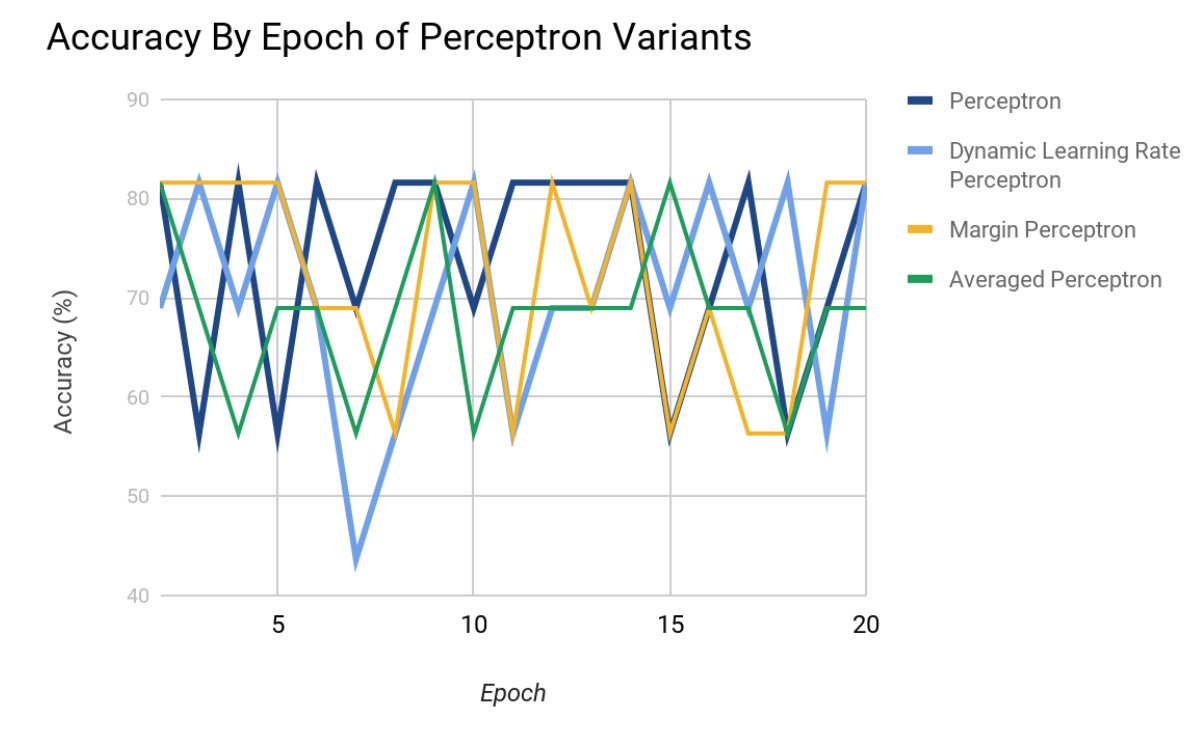
\includegraphics[width=12cm]{epoch.png}
\caption{Individual Epoch Accuracy}
\label{figure1}
\end{figure*}

\section{Methods and Implementation}
Our implementation was designed with the goal of predicting whether or not the home team would get a result from the game. In soccer, a team gets a result if they win or tie their opponent. We chose to predict whether or not the home team got a result because it allowed us to simplify the problem to binary classification. In addition, if we could accurately predict whether or not the home team gets a result, it would be trivial to extend the classifier to predict whether the away team gets a result. This in turn would allow us to predict the outcome of a game explicitly as a home win, tie, or home loss.

We used the Python programming language for our machine learning algorithms and for our feature extraction code. In an effort to explore the various tools and methodologies, we use various algorithms. The algorithms we used for this project included Support Vector Machines, Logistic Regression, variants of the Perceptron, Decision Trees, and Naive Bayes. We performed a grid search using 5-fold cross validation to tune hyper-parameters for each algorithm, such as learning rate and regularization terms. We then evaluated the performance of algorithm on a test set using the best set of hyper-parameters. For those models which train over epochs, the weights from the most successful epoch were used to evaluate against the test set.

We used various data sets to examine the results of each group. The MLS '16 dataset consists of the Major League Soccer games from the year 2016. This dataset was split into a training set that consisted of games from the first 90\% of the season, and a test set that consisted of games from the past 10\% of the season. The EPL '16 dataset consists of English Premier League matches from the year 2016. This dataset was also split into the first 90\% of games as training data and the last 10\% of games as test. The Random dataset consists of all the examples from every league and year. The Random dataset is split randomly between train and test sets, such that there is not consideration of time in the split. The impact of chronologically versus randomly split data is addressed in the evaluation. We also explore the impact of using the raw statistical features as opposed to the derived binary features.

\section{Evaluations}

\begin{table*}[t]
	\centering
        
        \begin{subtable}[h]{0.96\textwidth}
        \centering
        \begin{tabular}[h]{|>{\centering}m{4.5cm}>{\centering}m{4cm}>{\centering}m{2.5cm}c|}
        \hline
        Algorithm & Best Hyper-Parameters & Train Accuracy      & Test Accuracy\\ \hline \hline
        SVM & $r=10$, $C=10$ & 81.61\% & 81.08\%\\
        Logistic Regression & $r=1$, $C=1$ & 81.61\% & 81.08\%\\
        Perceptron & $r=0.01$ & 81.61\% & 81.08\%\\
        Dynamic Perceptron & $r=0.01$ & 81.61\% & 81.08\%\\ 
        Margin Perceptron & $r=0.01$, $\gamma=0.01$ & 81.61\% & 81.08\%\\ 
        Averaged Perceptron & $r=0.01$ & 68.06\% & 81.08\%\\\hline
        \end{tabular}
        \caption{MLS '16 Results}
        \label{table1a}
        \end{subtable}
        
        \begin{subtable}[h]{0.96\textwidth}
        \centering
        \begin{tabular}[h]{|>{\centering}m{4.5cm}>{\centering}m{4cm}>{\centering}m{2.5cm}c|}
        \hline
        Algorithm & Best Hyper-Parameters & Train Accuracy      & Test Accuracy\\ \hline \hline
        SVM & $r=10$, $C=0.01$ & 75.93\% & 83.33\%\\
        Logistic Regression & $r=1$, $C=100$ & 75.93\% & 83.33\%\\
        Perceptron & $r=0.01$ & 75.93\% & 83.33\%\\
        Dynamic Perceptron & $r=0.01$ & 67.77\% & 83.33\%\\ 
        Margin Perceptron & $r=0.01$, $\gamma=0.01$ & 75.93\% & 83.33\%\\ 
        Averaged Perceptron & $r=0.01$ & 66.30\% & 83.33\%\\\hline
        \end{tabular}
        \caption{EPL '16 Results}
        \label{table1b}
        \end{subtable}
        
        \begin{subtable}[h]{0.96\textwidth}
        \centering
        \begin{tabular}[h]{|>{\centering}m{4.5cm}>{\centering}m{4cm}>{\centering}m{2.5cm}c|}
        \hline
        Algorithm & Best Hyper-Parameters & Train Accuracy      & Test Accuracy \\ \hline \hline
        SVM & $r=1$, $C=10$ & 72.25\% & 75.30\%\\
        Logistic Regression & $r=1$, $C=1000$ &  72.25\% & 75.30\%\\
        Perceptron & $r=0.01$ &  72.25\% & 75.30\%\\
        Dynamic Perceptron & $r=0.01$ &  62.32\% & 75.30\%\\ 
        Margin Perceptron & $r=0.01$, $\gamma=0.01$ &  72.25\% & 75.30\%\\ 
        Averaged Perceptron & $r=0.01$ &  62.32\% & 75.30\%\\\hline
        \end{tabular}
        \caption{All Results}
        \label{table1c}
        \end{subtable}
        
        \caption{Evaluation Results}
        \label{table1}
\end{table*}

\subsection{Raw Features}
The results for running the algorithms on the various data sets using the raw statistical features are shown in Table \ref{table1}. The results for the MLS '16 data set, EPL '16 data set, and comprehensive data set are shown in Tables \ref{table1a} - \ref{table1c}, respectively. It is interesting to note, that the results largely show that each of the algorithms learns to simply predict that the home team gets a result. The majority label for each of the three data sets is that the home team gets a result, with percentages 81.08\%, 83.33\%, and 75.30\%, respectively. These curious results seemed to initially indicate errors in the implementation, such that the algorithms are simply guessing the majority label. However, for the SVM, logistic regression, and Perceptron variants, each algorithm is implemented twice, once by each author independently. The results are confirmed by running each set of algorithms against these data sets. Furthermore, the algorithms were run using other unrelated data sets, and non-trivial results are obtained. That is, the algorithms do not simply predict the majority label for other data sets in the same format. Nevertheless, we also rigorously inspected the code for errors, but found none. Thus, the results seem to indicate that the data and features have a significant impact on the performance of the algorithms. In addition, the results seem to show that the hypothesis spaces associated with our chosen algorithms are not expressive enough to manage the ``intangible'' elements of soccer and other sports.

Another interesting result which further shows the dependence on the data are the results of weights produced by individual epochs. Figure \ref{figure1} shows the accuracy of individual epochs for each algorithm over the MLS '16 data set. Rather than following a generally increasing path, the accuracy of successive epochs varies wildly, depending on the shuffling of data to start each epoch. This further indicates the importance of the impact of data on the results of the algorithms. 

\subsection{Derived Features}
Using the derived set of binary features over the whole data set, and training with the Naive Bayes and decision tree models, the algorithms output results similar to those above, achieving the test accuracy of 75.30\%. This continues to hold for using ensemble methods combining bagged forests with SVM and logistic regression. While we hoped that the derived features may be more expressive than the raw statistics, as noted in related work, the results don't appear promising. Unfortunately the results again indicate the data, features, and hypothesis spaces we are using are not expressive enough to capture the results of soccer matches.

\section{Future Work}
Because the classifiers trained on our data achieved their best performance by always predicting the home team would win, this suggests several possibilities that could influence future work. We would like to answer the question of whether or not being the home team really dominates all other aspects of the team's performance. If we found that the statistics we used to train our models did have predictive power regarding who will win the match, then we would investigate why our models were not able to effectively use these features. It is possible that the linear models we used had too much bias and not enough variance to capture the non-linear relationships in the data. However, it would be expected that the ensemble methods would have been able to capture these non-linear relationships.

There are many features we were unable to capture in our data like recent performance by each team, time since last match, injuries, trades, etc. It would be interesting to see if adding these features allows the model more predictive power. In addition, other high-level statistics could be found like goals per minute or considering performance against specific teams. It would be helpful to have more data as that could allow us to better overcome the natural noise and variance within sports. In addition, it would be a good idea to do more error checking on the data that was scraped and transformed into feature vectors to make sure there weren?t mistakes in the process.

\section{Conclusion}

\section*{Acknowledgements}
This report was completed for the course project in CS 5350: Machine Learning at the University of Utah in the Fall 2017 semester. We would like to acknowledge the help of Prof. Vivek Srikumar who taught us the principles and tools necessary to complete this project. Much of the implementation of different algorithms for this project was completed as part of assignments throughout the semester, and was modified to fit our needs for this project.

\bibliographystyle{ACM-Reference-Format}
\bibliography{bibliography} 

\end{document}
